%# -*- coding:utf-8 -*-
\documentclass[10pt,aspectratio=169,mathserif]{beamer}		
%设置为 Beamer 文档类型,设置字体为 10pt,长宽比为16:9,数学字体为 serif 风格

%%%%-----导入宏包-----%%%%
\usepackage{zju}			%导入 zju 模板宏包
%\usepackage{ctex}			%导入 ctex 宏包,添加中文支持
\usepackage{amsmath,amsfonts,amssymb,bm}   %导入数学公式所需宏包
\usepackage{color}			 %字体颜色支持
\usepackage{graphicx,hyperref,url}
\usepackage{metalogo}	% 非必须
%% 上文引用的包可按实际情况自行增删
%%%%%%%%%%%%%%%%%%
\usepackage{fontspec}
\usepackage{xeCJK}
% \setCJKmainfont{Source Han Sans SC}



\beamertemplateballitem		%设置 Beamer 主题

%%%%------------------------%%%%%
\catcode`\。=\active         %或者=13
\newcommand{。}{.}				
%将正文中的“。”号转换为“.”。中文标点国家规范建议科技文献中的句号用圆点替代
%%%%%%%%%%%%%%%%%%%%%

%%%%----首页信息设置----%%%%
\title[Optimization of Corner Blending Curves]{Optimization of Corner Blending Curves}
%\subtitle{——这里是副标题}			
%%%%----标题设置


\author[WSL]{
   Rida T. Farouki , Francesca Pelosi, Maria Lucia Sampoli \\\medskip
  {\small {Department of Mechanical and Aerospace Engineering, University of California\\
  		Dipartimento di Matematica, Università di Roma "Tor Vergata", Via della Ricerca Scientifica\\
  		Dipartimento di Ingegneria dell'Informazione e Scienze Matematiche, Università di Siena}} \\
 }
%%%%----个人信息设置
  
%\institute[IOPP]{
 % 计算机学院 \\ 
  %浙江大学}
%%%%----机构信息

\date[Apr. 29 2025]{
  2025.4.29}
%%%%----日期信息
  
\begin{document}

\begin{frame}
	\titlepage
\end{frame}				%生成标题页


\begin{frame}
	\frametitle{Contents}
	\tableofcontents
\end{frame}				%生成提纲页

\section{Introduction}
\begin{frame}
	\frametitle{Introduction}
	 
	
\end{frame}

\section{Canonical corner blending problem}
\begin{frame}
	\frametitle{Canonical corner blending problem}
	See the figure below, we have
	$\mathbf{p}_i=(-1,0)\:,\quad\mathbf{p}_c=(0,0)\:,\quad\mathbf{p}_o=(\cos\theta,\sin\theta)\:$ and 
	 $$\|\mathbf{p}_c-\mathbf{p}_i\|=\|\mathbf{p}_o-\mathbf{p}_c\|$$
 $\mathbf{t}(0)=\mathbf{r}^{\prime}(0)/\|\mathbf{r}^{\prime}(0)\|=(1,0)$ and t(1)= $\mathbf{r} ^{\prime }( 1) / \| \mathbf{r} ^{\prime }( 1) \|$ = $( \cos \theta , \sin \theta ) .$ 
	The parametric speed of the curve r$(\xi)=(x(\xi),y(\xi))$ is defined
	by
	$$\sigma(\xi)\:=\:\left\|\mathbf{r}'(\xi)\right\|\:=\:\sqrt{x'^2(\xi)+y'^2(\xi)}\:=\:\frac{\mathrm{d}s}{\mathrm{d}\xi}\:,$$
	where s is arc length along r($\xi).$
	\begin{figure}
		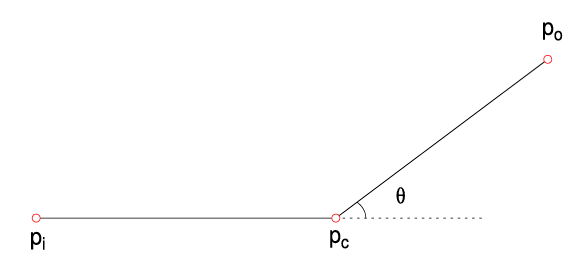
\includegraphics[scale=0.4]{figures/1.png}
	\end{figure}
	
\end{frame}

\begin{frame}
	\frametitle{Canonical corner blending problem}
	In the context of applications, two features of the corner rounding curve are of particular interest — the deviation $\delta_m$ of the mid-point from the original exact corner $(0 , 0)$ and the mid-point
	curvature magnitude, namely
	$$\delta_{\mathrm{m}}=\parallel\mathbf{r}(\frac{1}{2})\parallel\quad\mathrm{and}\quad\kappa_{\mathrm{m}}=\mid\kappa(\frac{1}{2})\mid.$$
	The goal is thus to identify smooth curves, satisfying prescribed continuity conditions at $p_i$ and $p_o$, that balance the desire to subdue both $\delta_m$ and $\kappa_m$.
	
	\begin{figure}
		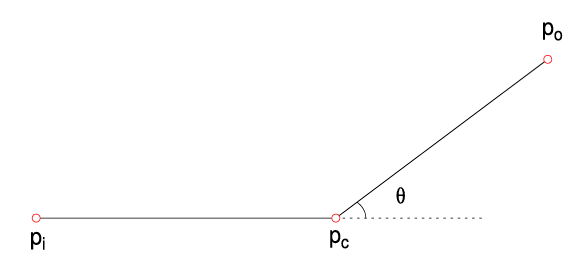
\includegraphics[scale=0.4]{figures/1.png}
	\end{figure}
	
\end{frame}

\section{Polynomial corner curves}
\begin{frame}
	\frametitle{Polynomial corner curves}
	Consider the use of a planar degree $n$ Bézier curve
	
	$$\mathbf{r}(\xi)\:=\:\sum_{k=0}^{n}\mathbf{p}_{k}\:b_{k}^{n}(\xi)\:,\quad b_{k}^{n}(\xi)\:=\:\binom{n}{k}(1-\xi)^{n-k}\xi^{k}\:,$$
	
	symmetric about the normal line at the mid-point $\mathbf{r}(\frac{1}{2})$ to define a corner curve. For even $n$, we set
	$$\mathbf{p}_{0}\:=\:\mathbf{p}_{i}\:,\quad\mathbf{p}_{n/2}\:=\:\mathbf{p}_{c}\:,\quad\mathbf{p}_{n}\:=\:\mathbf{p}_{o}\:,$$
	and for odd $n$, we again set $\mathbf{p}_0 = \mathbf{p}_i$
	and $\mathbf{p}_n = \mathbf{p}_o$.
\end{frame}

\begin{frame}
	\frametitle{Polynomial corner curves(The case $n=3$)}

		$$\mathbf{p}_{0}\:=\:(-1,0)\:,\quad\mathbf{p}_{1}\:=\:\lambda(-1,0)\:\:\mathbf{p}_{2}\:=\:\lambda(\cos\theta,\sin\theta)\:,\quad\mathbf{p}_{3}\:=\:(\cos\theta,\sin\theta)\:.$$
		
		$$\delta_{\mathrm{m}}\:=\:\frac{|\sin\frac{1}{2}\theta\:|}{4}\:(3\lambda+1)\:,\quad\kappa_{\mathrm{m}}\:=\:\frac{8\sqrt{2}\:|\sin\theta\:|}{3(1+\cos\theta)^{3/2}}\:\frac{1-\lambda}{(1+\lambda)^2}.$$
		\begin{columns}
			\column{0.4\textwidth}
			\begin{figure}[htbp]
				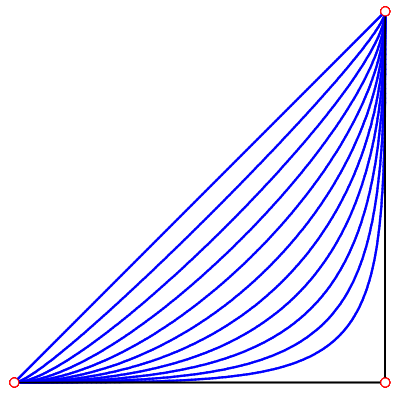
\includegraphics[scale=0.27]{figures/2.png}
			\end{figure}
		\column{0.6\textwidth}
		Note that $\delta_ m$ is monotone-increasing with $\lambda$, having its minimum value when $\lambda = 0$ with $\mathbf{p}_1 = \mathbf{p}_2 = (0 , 0)$. \\
		On the other hand, $\kappa_m$
		is monotone-decreasing with $\lambda$ , having its minimum value when
		$\lambda = 1$with $\mathbf{p}_0 = \mathbf{p}_1 = ( − 1 , 0)$ and $\mathbf{p}_2 = \mathbf{p}_3 = (\cos \theta, \sin \theta )$.
		Figure left shows examples of these degree 3 corner curves for the
		turning angle $\theta=\pi/2$.
		\end{columns}
\end{frame}

\begin{frame}
	\frametitle{Polynomial corner curves(The case $n=4$)}
	
	$$\mathbf{p}_{0}\:=\:(-1,0)\:,\quad\mathbf{p}_{1}\:=\:\lambda(-1,0)\:,\quad \mathbf{p}_{2}\:=\:(0,0)\:,\quad\mathbf{p}_{3}\:=\:\lambda(\cos\theta,\sin\theta)\:,\quad\mathbf{p}_{4}\:=\:(\cos\theta,\sin\theta)\:.$$
	
	$$\delta_{\mathrm{m}}\:=\:\frac{|\sin\frac{1}{2}\theta\:|}{8}\:(4\lambda+1)\:,\quad\kappa_{\mathrm{m}}\:=\:\frac{6\sqrt{2}\:|\sin\theta\:|}{(1+\cos\theta)^{3/2}}\:\frac{1}{(1+2\lambda)^2}.$$
	\begin{columns}
		\column{0.4\textwidth}
		\begin{figure}[htbp]
			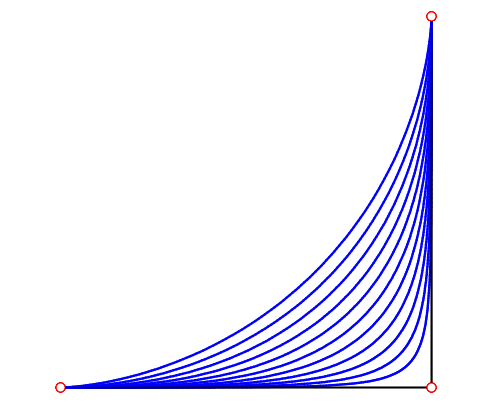
\includegraphics[scale=0.27]{figures/3.png}
		\end{figure}
		\column{0.6\textwidth}
		As in the case $n=3$, $\delta_{m}$ is monotone-increasing with $\lambda$ , having its minimum value when $\lambda=0$ with $\mathbf{p} _{1}$ = $\mathbf{p} _{2} = \mathbf{p}_{3}=(0,0)$ , whereas $\kappa_{\mathrm{m}}$ is monotone-decreasing with $\lambda$ ,having its minimum value when $\lambda=1$ with $\mathbf{p}_{0}=\mathbf{p}_{1}=(-1,0)$ and $\mathbf{p}_{2}=\mathbf{p}_{3}=(\cos\theta,\sin\theta)$.
		
	\end{columns}
\end{frame}

\begin{frame}
	\frametitle{Polynomial corner curves(The case $n=5$)}
	To achieve a $G^2$ connection using a quintic curve, the control
	points $\mathbf{p}_0,\mathbf{p}_1,\mathbf{p}_2$ must be co-linear, and $ \mathbf{p}_3,\mathbf{p}_4,\mathbf{p}_5$ must be co-linear—i.e.,we must have
	$$\begin{aligned}&\mathbf{p}_{0}\:=\:(-1,0)\:,\quad\mathbf{p}_{1}\:=\:\lambda(-1,0)\:,\quad\mathbf{p}_{2}\:=\:\mu(-1,0)\:,\\&\mathbf{p}_{3}\:=\:\mu(\cos\theta,\sin\theta)\:,\quad\mathbf{p}_{4}\:=\:\lambda(\cos\theta,\sin\theta)\:,\\&\mathbf{p}_{5}\:=\:(\cos\theta,\sin\theta)\:,\end{aligned}$$
	
	$\lambda,\mu\in[0,1]$ being free parameters with $\lambda\geq\mu.$
	
	$$\begin{aligned}&\delta_{\mathrm{m}}\:=\:\frac{\left|\sin\frac{1}{2}\theta\right|}{16}\left(5\:\lambda+10\:\mu+1\right),\\&\kappa_{\mathrm{m}}\:=\:\frac{64\sqrt{2}\left|\sin\theta\right|}{5\left(1+\cos\theta\right)^{3/2}}\frac{\lambda-2\:\mu+1}{(3\:\lambda+2\:\mu+1)^{2}}\:.\end{aligned}$$
	
	
\end{frame}
\begin{frame}
	\frametitle{Polynomial corner curves(The case $n=6$)}
	To achieve a $G^3$ connection with the incoming/outgoing linear segments, we must have $\kappa(0)=$ d$\kappa/$ds(1)=0 and $\kappa(1)=$ d$\kappa/$ds(0)=0. We must have
	
	$$\begin{aligned}&\mathbf{p}_{0}=(-1,0),\quad\mathbf{p}_{1}=\lambda(-1,0),\\&\mathbf{p}_{2}=\mu(-1,0),\quad\mathbf{p}_{3}=(0,0),\\&\mathbf{p}_{4}=\mu(\cos\theta,\sin\theta),\quad\mathbf{p}_{5}=\lambda(\cos\theta,\sin\theta),\\&\mathbf{p}_{6}=(\cos\theta,\sin\theta),\end{aligned}$$
	$\lambda,\mu\in[0,1]$ being free parameters with $\lambda\geq\mu.$ 
	$$\begin{aligned}&\delta_{\mathrm{m}}\:=\:\frac{|\sin\frac{1}{2}\theta\:|}{32}\:(6\:\lambda+15\:\mu+1)\:,\\&\kappa_{\mathrm{m}}\:=\:\frac{80\sqrt{2}\left|\sin\theta\right|}{3(1+\cos\theta)^{3/2}}\frac{2\:\lambda-\mu+1}{(4\:\lambda+5\:\mu+1)^{2}}\:.\end{aligned}$$
	
	
\end{frame}
\section{Corner curve optimization}
\begin{frame}
	\frametitle{Corner curve optimization}
	The arc length $S$ of the corner curve $r( \xi)$ is defined in terms of the
	parametric speed by
	$$S = \int_0^1\sigma(\xi)\mathrm{d}\xi$$
	and the mean value of ${\sigma} ( \xi )$ is $\overline{\sigma}= S$. A dimensionless measure
	of the mean square deviation of $\sigma ( \xi )$ about $\overline{\sigma}$ is then defined through the expression
	$$\gamma = \frac1{S^2}\int_0^1[\sigma(\xi)-\overline{\sigma}]^2\mathrm{d}\xi=\frac1{S^2}\int_0^1\sigma^2(\xi)-1$$
\end{frame}
\begin{frame}
	\frametitle{Corner curve optimization}
We introduce individual dimensionless measures of $\kappa_\mathrm{m}$ and $\delta_{m}$ by dividing them by the values
$$\bar{\kappa}_{\mathrm{m}}\:=\:\frac{\mid\theta\mid}{S}\quad\mathrm{and}\quad\bar{\delta}_{\mathrm{m}}\:=\:\frac{1}{2}\mid\sin\frac{1}{2}\theta\mid.$$
These are the averages of $\kappa_{\mathrm{m}}$ and $\delta_{\mathrm{m}}$ for the two "extreme" solutions identified, namely, the piecewise-linear path from $\mathbf{p}_i$ to $\mathbf{p}_o$ through $\mathbf{p}_o$, and the direct short-cut linear path from $\mathbf{p}_i$ to $\mathbf{p}_o$. We then define the objective function
$$f = a(\delta_{\mathrm{m}}/\bar{\delta}_{\mathrm{m}})+b(\kappa_{\mathrm{m}}/\bar{\kappa}_{\mathrm{m}})+(1-a-b)\gamma$$
where $a, b$ are non-negative weights such that $a + b \leq 1$.
\end{frame}
\section{Optimization algorithm}
\begin{frame}
	\frametitle{Univariate objective function}
	
\end{frame}
\section{Computed examples}
\begin{frame}
	\frametitle{Computed examples}
	\begin{columns}
		\column{0.45\textwidth}
		$$f = a(\delta_{\mathrm{m}}/\bar{\delta}_{\mathrm{m}})+b(\kappa_{\mathrm{m}}/\bar{\kappa}_{\mathrm{m}})+(1-a-b)\gamma$$
		$$\gamma = \frac1{S^2}\int_0^1[\sigma(\xi)-\overline{\sigma}]^2\mathrm{d}\xi=\frac1{S^2}\int_0^1\sigma^2(\xi)-1$$
		
		\begin{figure}
			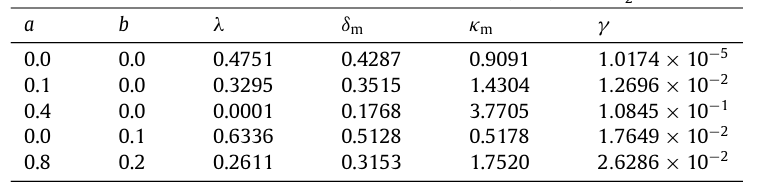
\includegraphics[scale=0.5]{figures/4.png}
			\caption{Numerical results for cubic corner curves with turning angle $\theta=\frac\pi2$.}
		\end{figure}
		\column{0.55\textwidth}
		\begin{figure}
			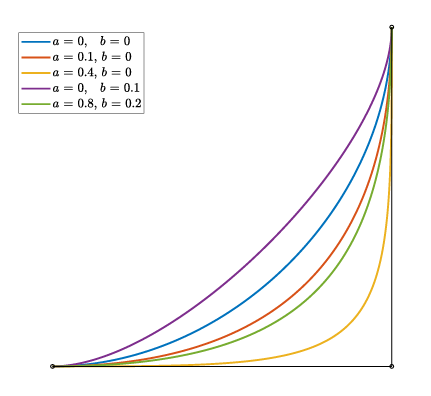
\includegraphics[scale=0.6]{figures/5.png}
		\end{figure}
	\end{columns}
\end{frame}
\begin{frame}
	\frametitle{Computed examples}
	\begin{columns}
		\column{0.5\textwidth}
		\begin{figure}
			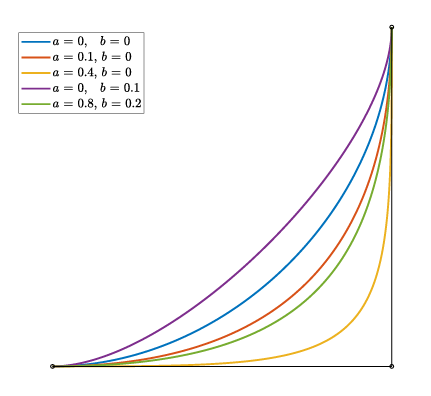
\includegraphics[scale=0.5]{figures/5.png}
		\end{figure}
		\column{0.5\textwidth}
		\begin{figure}
			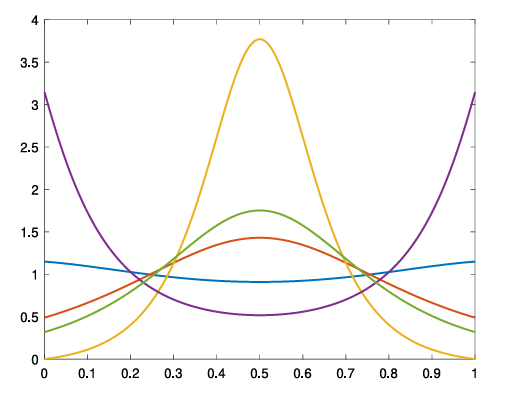
\includegraphics[scale=0.5]{figures/6.png}
		\end{figure}
	\end{columns}
\end{frame}
\begin{frame}
	\frametitle{Computed examples}
	\begin{columns}
		\column{0.45\textwidth}
		$$f = a(\delta_{\mathrm{m}}/\bar{\delta}_{\mathrm{m}})+b(\kappa_{\mathrm{m}}/\bar{\kappa}_{\mathrm{m}})+(1-a-b)\gamma$$
		$$\gamma = \frac1{S^2}\int_0^1[\sigma(\xi)-\overline{\sigma}]^2\mathrm{d}\xi=\frac1{S^2}\int_0^1\sigma^2(\xi)-1$$
		
		\begin{figure}
			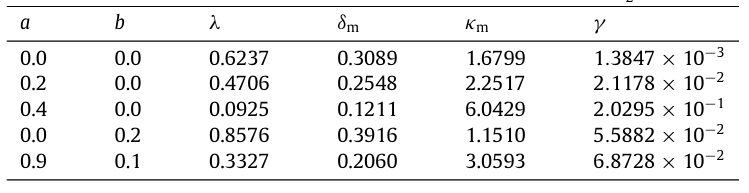
\includegraphics[scale=0.5]{figures/8.png}
			\caption{Numerical results for quartic corner curves with turning angle $\theta=\frac\pi2$.}
		\end{figure}
		\column{0.55\textwidth}
		\begin{figure}
			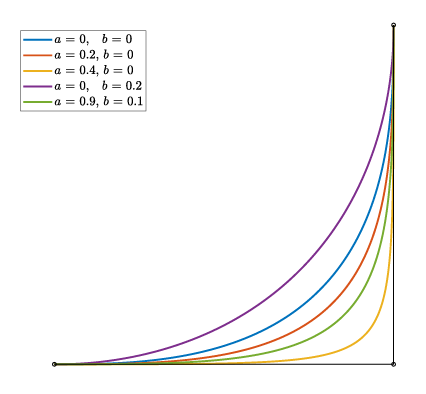
\includegraphics[scale=0.6]{figures/7.png}
		\end{figure}
	\end{columns}
\end{frame}
\begin{frame}
	\frametitle{Computed examples}
	\begin{columns}
		\column{0.5\textwidth}
		\begin{figure}
			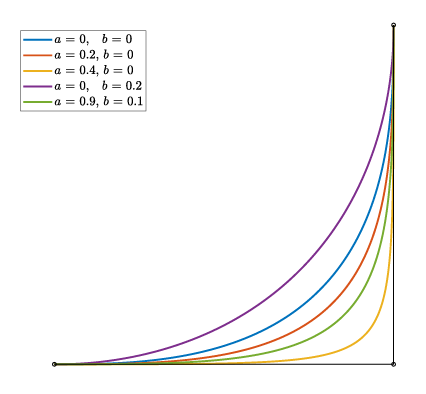
\includegraphics[scale=0.5]{figures/7.png}
		\end{figure}
		\column{0.5\textwidth}
		\begin{figure}
			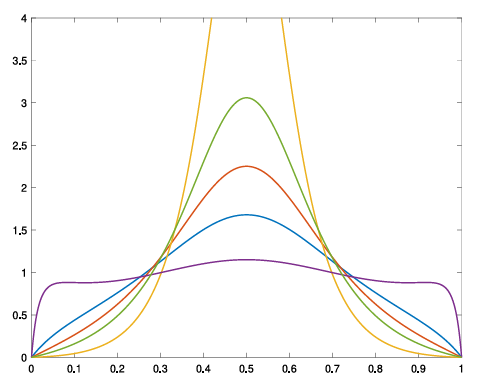
\includegraphics[scale=0.5]{figures/9.png}
		\end{figure}
	\end{columns}
\end{frame}
\begin{frame}
	\frametitle{Computed examples}
	\begin{columns}
		\column{0.45\textwidth}
		$$f = a(\delta_{\mathrm{m}}/\bar{\delta}_{\mathrm{m}})+b(\kappa_{\mathrm{m}}/\bar{\kappa}_{\mathrm{m}})+(1-a-b)\gamma$$
		$$\gamma = \frac1{S^2}\int_0^1[\sigma(\xi)-\overline{\sigma}]^2\mathrm{d}\xi=\frac1{S^2}\int_0^1\sigma^2(\xi)-1$$
		
		\begin{figure}
			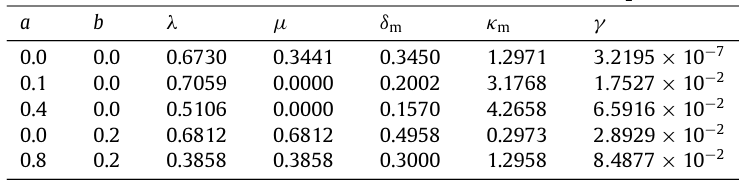
\includegraphics[scale=0.5]{figures/12.png}
			\caption{Numerical results for quintic corner curves with turning angle $\theta=\frac\pi2$.}
		\end{figure}
		\column{0.55\textwidth}
		\begin{figure}
			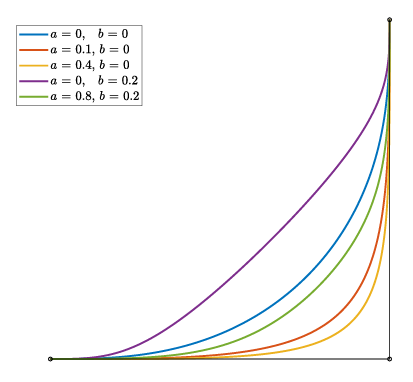
\includegraphics[scale=0.6]{figures/10.png}
		\end{figure}
	\end{columns}
\end{frame}
\begin{frame}
	\frametitle{Computed examples}
	\begin{columns}
		\column{0.5\textwidth}
		\begin{figure}
			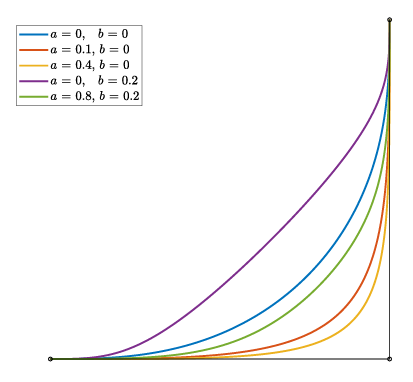
\includegraphics[scale=0.5]{figures/10.png}
		\end{figure}
		\column{0.5\textwidth}
		\begin{figure}
			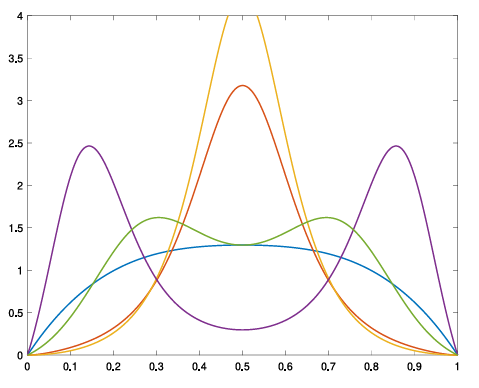
\includegraphics[scale=0.5]{figures/11.png}
		\end{figure}
	\end{columns}
\end{frame}
\end{document}